\documentclass[a4paper,12pt]{article} % тип документа

% Поля страниц
\usepackage[left=2.5cm,right=2.5cm,
    top=2cm,bottom=2cm,bindingoffset=0cm]{geometry}
    
%Пакет дял таблиц   
\usepackage{multirow} 
    
%Отступ после заголовка    
\usepackage{indentfirst}


% Рисунки
\usepackage{floatrow,graphicx,calc}
\usepackage{wrapfig}

%%% Работа с картинками
\usepackage{graphicx}  % Для вставки рисунков
\graphicspath{{images/}{images2/}}  % папки с картинками
\setlength\fboxsep{3pt} % Отступ рамки \fbox{} от рисунка
\setlength\fboxrule{1pt} % Толщина линий рамки \fbox{}
\usepackage{wrapfig} % Обтекание рисунков и таблиц текстом

% Создаёем новый разделитель
\DeclareFloatSeparators{mysep}{\hspace{1cm}}

% Ссылки?
\usepackage{hyperref}
\usepackage[rgb]{xcolor}
\hypersetup{				% Гиперссылки
    colorlinks=true,       	% false: ссылки в рамках
	urlcolor=blue          % на URL
}


%  Русский язык
\usepackage[T2A]{fontenc}			% кодировка
\usepackage[utf8]{inputenc}			% кодировка исходного текста
\usepackage[english,russian]{babel}	% локализация и переносы




% Математика
\usepackage{amsmath,amsfonts,amssymb,amsthm,mathtools}

%%% Дополнительная работа с математикой
\usepackage{amsmath,amsfonts,amssymb,amsthm,mathtools} % AMS
\usepackage{icomma} % "Умная" запятая: $0,2$ --- число, $0, 2$ --- перечисление


% Что-то 
\usepackage{wasysym}


\begin{document}
\begin{center}
	\footnotesize{ФЕДЕРАЛЬНОЕ ГОСУДАРСТВЕННОЕ АВТОНОМНОЕ ОБРАЗОВАТЕЛЬНОЕ 			УЧРЕЖДЕНИЕ ВЫСШЕГО ОБРАЗОВАНИЯ}\\
	\footnotesize{МОСКОВСКИЙ ФИЗИКО-ТЕХНИЧЕСКИЙ ИНСТИТУТ\\(НАЦИОНАЛЬНЫЙ 			ИССЛЕДОВАТЕЛЬСКИЙ УНИВЕРСИТЕТ)}\\
	\footnotesize{ФАКУЛЬТЕТ ОБЩЕЙ И ПРИКЛАДНОЙ ФИЗИКИ\\}
	\hfill \break
	\hfill \break
	\hfill \break
	\hfill \break
\end{center}


\begin{figure*}[h]
    \centering
    \includegraphics*[width=10cm,height=7cm,keepaspectratio]{mipt_eng_text_png.png}
    \label{fig:my_label}
\end{figure*}


\begin{center}   
    \hfill \break
	\hfill \break
	\hfill \break
	\hfill \break
	\large{Лабораторная работа № 2.1.3\\\textbf{Определение $\displaystyle C_p/C_v$ по скорости звука в газе}}\\
	\hfill \break
	\hfill \break
	\hfill \break
	\hfill \break
	\begin{flushright}
		Баранов Даниил\\
		Группа Б02-103
	\end{flushright}
	\hfill \break
	\hfill \break
	\hfill \break
\end{center}
\hfill \break
\hfill \break
\hfill \break
\hfill \break
\begin{center}
	Долгопрудный, 2022 г.
\end{center}
\thispagestyle{empty}



\newpage

\textbf{Цель работы:} 1) измерение частоты колебаний и длины волны при резонансе звуковых колебаний в газе, заполняющем трубу; 2) определение показателя адиабаты с помощью уравнения состояния идеального газа.\hfill
\break
	
\textbf{В работе используются:} звуковой генератор; электонный осциллограф; микрофон; телефон; раздвижная труба; теплоизолированная труба, обогреваемая водой из термостата; баллон со сжатым углекислым газом.

\section{Теоритеческая часть}

Скорость распространения звуковой волны в газах зависит от показателя адиабаты $ \gamma $. На измерении скорости звука основан один из наиболее точных методов определения показателя адиабаты.

Скорость звука в газах определяется формулой:

\begin{equation}
\label{velocity}
c=\sqrt{\gamma\frac{RT}{\mu}}
\end{equation}
где $ R $ -- газовая постоянная, $ T $ -- температура газа, а $ \mu $ -- его молярная масса. Преобразуя эту формулу, найдем
\begin{equation}
\label{gamma}
\gamma = \frac{\mu}{RT}c^2
\end{equation}

Таким образом, для определения показателя адиабаты достаточно измерить температуру газа и скорость распространения звука (молярная масса газа предполагается известной).

Звуковая волна, распространяющаяся вдоль трубы, испытывает многократные отражения от торцов. Звуковые колебания в трубе являются наложением всех отраженных волн и очень сложны. Картина упрощается, если длина трубы $ L $ равна целому числу полуволн, то есть когда
\[
L=\frac{n\lambda}{2}
\] где $ \lambda $ -- длина волны звука в трубе, а $ n $ -- любое целое число. Если это условие выполнено, то волна, отраженная от торца трубы, вернувшаяся к ее началу и вновь отраженная, совпадает по фазе с падающей. Совпадающие по фазе волны усиливают друг друга. Амплитуда звуковых колебаний при этом резко возрастает -- наступает резонанс.

При звуковых колебаниях слои газа, прилегающие к торцам трубы, не испытывают смещения. Узлы смещения повторяются по всей длине трубы через $ \lambda/2 $. Между узлами находятся максимумы смещения.

Скорость звука c связана с его частотой $ f $ и длиной волны $ \lambda $ соотношением

\begin{equation}\label{lambda_f}
c=\lambda f
\end{equation}

Подбор условий, при которых возникает резонанс, можно производить двояко:
\begin{enumerate}
\item При неизменной частоте $ f $ звукового генератора (а следовательно, и неизменной длине звуковой волны $ \lambda $) можно изменять длину трубы $ L $. Для этого применяется раздвижная труба. Длина раздвижной трубы постепенно увеличивается, и наблюдается ряд последовательных резонансов. Возникновение резонанса легко наблюдать на осциллографе по резкому увеличению амплитуды колебаний. Для последовательных резонансов имеем
\begin{equation}\label{first}
L_n=n\frac{\lambda}{2}, \quad L_{n+1}=(n+1)\frac{\lambda}{2}, \quad \dots, \quad L_{n+k} = n\frac{\lambda}{2}+k\frac{\lambda}{2},
\end{equation} т. е. $ \lambda/2 $ равно угловому коэффициенту графика, изображающего зависимость длины трубы $ L $ от номера резонанса $ k $. Скорость звука находится по формуле \eqref{lambda_f}.
\item При постоянной длине трубы можно изменять частоту звуковых колебаний. В этом случае следует плавно изменять частоту $ f $ звукового генератора, а следовательно, и длину звуковой волны $ \lambda $. Для последовательных резонансов получим 
\begin{equation}\label{4}
L=\frac{\lambda_1}{2}n=\frac{\lambda_2}{2}(n+1)=\dots=\frac{\lambda_{k+1}}{2}(n+k).
\end{equation}

Из \eqref{lambda_f} и \eqref{4} имеем:
\[ f_1=\frac{c}{\lambda_1}=\frac{c}{2L}n, \quad f_2=\frac{c}{\lambda_2}=\frac{c}{2L}(n+1)=f_1+\frac{c}{2L},\quad \dots, \]
\begin{equation}\label{5}
f_{k+1}=\frac{c}{\lambda_{k+1}}=\frac{c}{2L}(n+k)=f_1+\frac{c}{2L}k.
\end{equation}
Скорость звука, деленная на $ 2L $, определяется, таким образом, по угловому коэффициенту графика зависимости частоты от номера резонанса.
\end{enumerate}

\section{Экспериментальная установка}

Соответственно двум методам измерения скорости звука в работе имеются две установки (рис. \ref{img1} и \ref{img2}). В обеих установках звуковые колебания в трубе возбуждаются телефоном Т и улавливаются микрофоном М. Мембрана телефона приводится в движение переменным током звуковой частоты; в качестве источника переменной ЭДС используется звуковой генератор ГЗ. Возникающий в микрофоне сигнал наблюдается на осциллографе ЭО.

Микрофон и телефон присоединены к установке через тонкие резиновые трубки. Такая связь достаточна для возбуждения и обнаружения звуковых колебаний в трубе и в то же время мало возмущает эти колебания: при расчетах оба торца трубы можно считать неподвижными, а влиянием соединительных отверстий пренебречь.

Первая установка (рис. \ref{img1}) содержит раздвижную трубу с миллиметровой шкалой. Через патрубок (на рисунке не показан) труба может наполняться воздухом или углекислым газом из газгольдера. На этой установке производятся измерения $ \gamma $ для воздуха и для $ CO_2 $. Вторая установка (рис. \ref{img2}) содержит теплоизолированную трубу постоянной длины. Воздух в трубе нагревается водой из термостата. Температура газа принимается равной температуре омывающей трубу воды. На этой установке измеряется зависимость скорости звука от температуры.

\begin{figure}[H]
	\begin{center}
		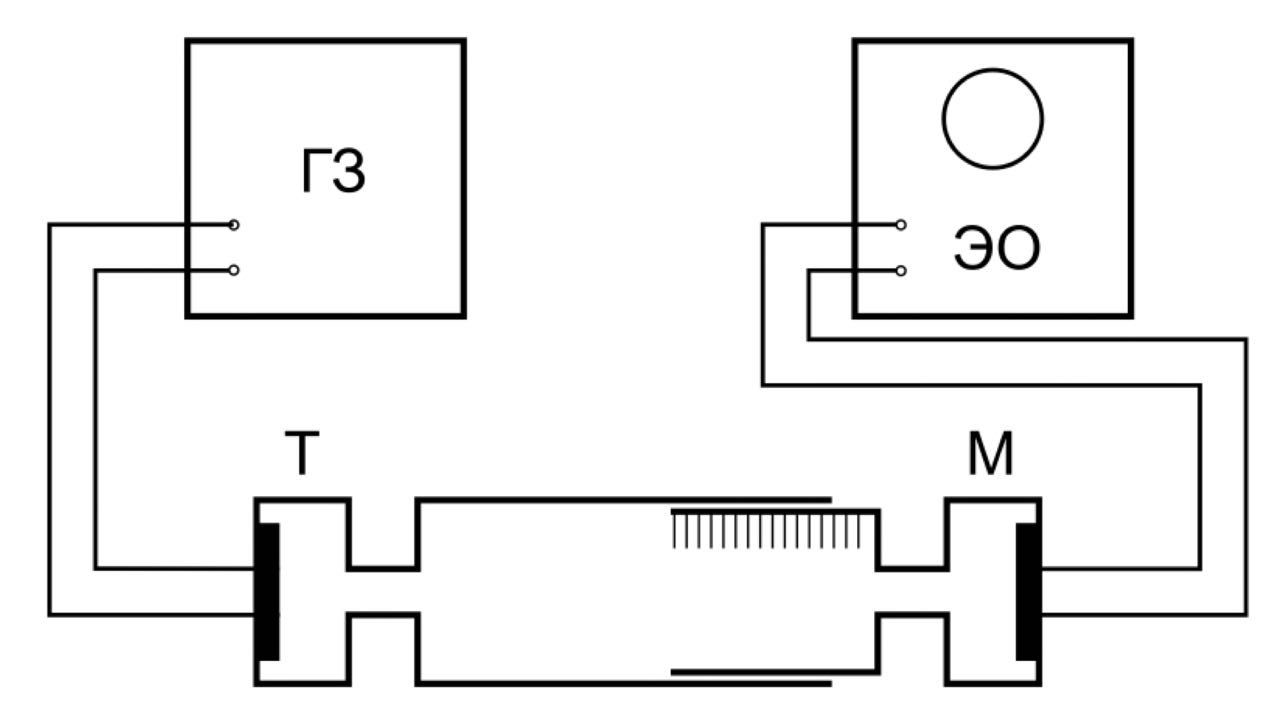
\includegraphics[width=12cm]{ust1.jpg}
	\end{center}
	\caption{Установка для измерения скорости звука при помощи раздвижной трубы}
	\label{img1}
\end{figure}

\begin{figure}[H]
	\begin{center}
		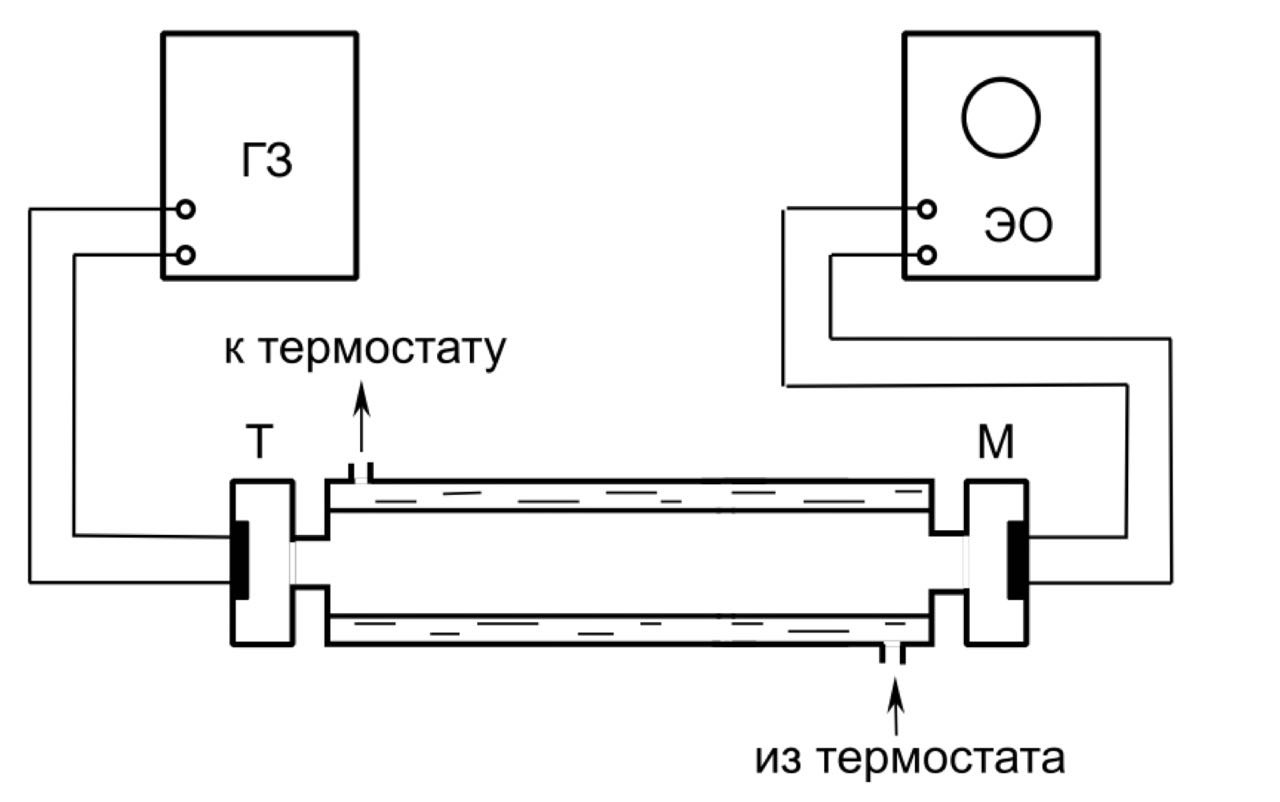
\includegraphics[width=12cm]{ust2.jpg}
	\end{center}
	\caption{Установка для изучения зависимости скорости звука от температуры}
	\label{img2}
\end{figure}

\section{Результаты измерений}

Проведём измерение коэффициента $ C_p/C_v $ для воздуха при помощи установки с раздвижной трубой. Для проведения серии измерений фиксируем частоту звукового сигнала и оставляем её неизменной до окончания снятия показаний. Увеличиваем и уменьшаем длину трубки, чтобы добиться резонанса, возникновение которого устанавливается при помощи осциллографа. При возникновении резонанса фиксируем то расстояние, на которое была выдвинута трубка прибора. Данные измерения проводим для нескольких значений частот. Полученные результаты заносим в таблицу 1. Все измерения проводились при температуре в комнате $T=297.5K$

\begin{table}[h]
    \begin{tabular}{|p{2cm}|p{2cm}|p{2cm}|p{2cm}|p{2cm}|p{2cm}|}
    \hline
    \multicolumn{6}{|c|}{Воздух, $L = 575$ мм} \\ \hline
    \nu,\ \text{кГц} & 2 & 3 & 4 & 5 & 6 \\ \hline
    $\Delta L_1$, мм & 31  & 4   & 34  & 16  & 6 \\ \hline
    $\Delta L_2$, мм & 118 & 62  & 77  & 52  & 36 \\ \hline
    $\Delta L_3$, мм & 203 & 119 & 121 & 86  & 65 \\ \hline
    $\Delta L_4$, мм & --  & 177 & 162 & 122 & 94 \\ \hline
    $\Delta L_5$, мм & --  & --  & 207 & 156 & 123 \\ \hline
    $\Delta L_6$, мм & --  & --  & --  & 191 & 151 \\ \hline
    \multicolumn{6}{}{} \\ \hline
    \multicolumn{6}{|c|}{$CO_2$, $L = 575$ мм} \\ \hline
    \nu,\ \text{кГц} & 2 & 3 & 4 & 5 & 6 \\ \hline
    $\Delta L_1$, мм & 38  & 8   & 7   & 30  & -- \\ \hline
    $\Delta L_2$, мм & 108 & 61  & 43  & 57  & -- \\ \hline
    $\Delta L_3$, мм & 181 & 113 & 80  & 92  & -- \\ \hline
    $\Delta L_4$, мм & --  & 174 & 116 & 115 & -- \\ \hline
    $\Delta L_5$, мм & --  & --  & 154 & 141 & -- \\ \hline
    $\Delta L_6$, мм & --  & --  & 195 & 172 & -- \\ \hline
    \end{tabular}
    \label{oxy}
    \caption {Увеличение длины трубы при резонансе}
\end{table}

Средняя погрешность измеренной длины составила $\sigma_L\approx 1$ мм.

Проведём измерения $ C_p/C_v $ для воздуха при различных температурах. Для этого будем использовать трубу постоянного размера $L = 700 \pm 1$ мм. Для фиксированной температуры будем изменять частоту звукового сигнала, тем самым изменяя и длину волны, так, чтобы мы могли наблюдать последовательные резонансы. Для каждого резонанса будем фиксировать частоту, при которой он возник. Полученные измерения занесём в таблицу 2.

\begin{table}[h]
    \begin{tabular}{|p{2cm}|p{2cm}|p{2cm}|p{2cm}|p{2cm}|p{2cm}|}
    \hline
    \multicolumn{2}{|c|}{$t=23^\circ C$} & \multicolumn{2}{|c|}{$t=35^\circ C$} & \multicolumn{2}{|c|}{$t=50^\circ C$} \\ \hline
    k & \nu_{\text{рез}}, \text{Гц} & k & \nu_{\text{рез}}, \text{Гц} & k & \nu_{\text{рез}}, \text{Гц} \\ \hline
    1 & 264  & 1 & 263  & 1 & 275  \\ \hline
    2 & 498  & 2 & 507  & 2 & 519  \\ \hline
    3 & 741  & 3 & 755  & 3 & 773  \\ \hline
    4 & 989  & 4 & 1009 & 4 & 1031 \\ \hline
    5 & 1235 & 5 & 1259 & 5 & 1288 \\ \hline
    6 & 1480 & 6 & 1509 & 6 & 1543 \\ \hline
    7 & 1727 & 7 & 1753 & 7 & 1799 \\ \hline
    8 & 1976 & 8 & 2013 & 8 & 2061 \\ \hline
    9 & 2218 & 9 & 2260 & 9 & 2312 \\ \hline
    \end{tabular}
    \label{tab:constL}
    \caption {\centering Результаты измерений резонансной частоты при разных температурах и числу полуволн}
\end{table}

Максимальная погрешность измеренной частоты оказалась равной $\sigma_{\nu}\approx3$ Гц.

\section{Обработка полученных данных}

По данным таблицы 1 построим графики (\ref{fig:air} и \ref{fig:CO}) зависимости удлинения трубы от номера полученного резонанса, считая первое удлинение соответствующим первому резонансу (вычитание константы не меняет наклон графика).

\begin{figure}[H]
	\begin{center}
		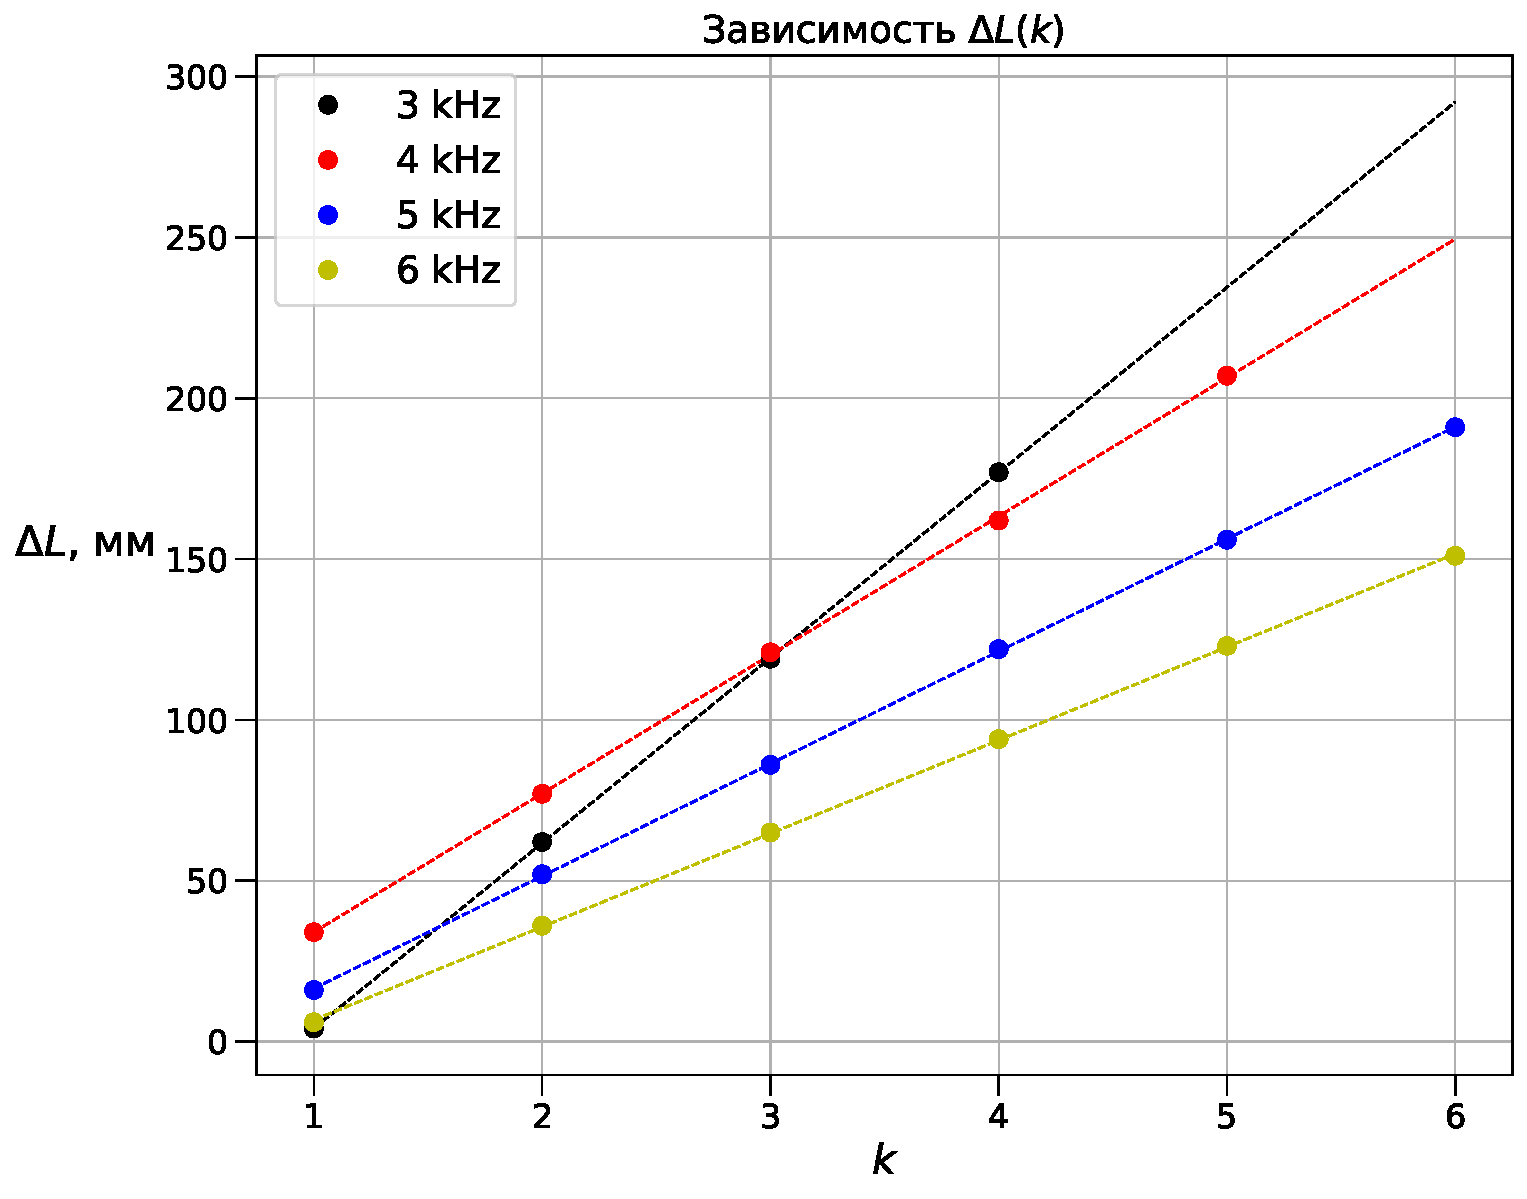
\includegraphics[scale=0.65]{2.1.3/L(k).pdf}
		\caption{\centering График зависимости удлинения трубы от \\ номера полученного резонанса для воздуха}
		\label{fig:air}
	\end{center}
\end{figure}

\begin{figure}[H]
	\begin{center}
		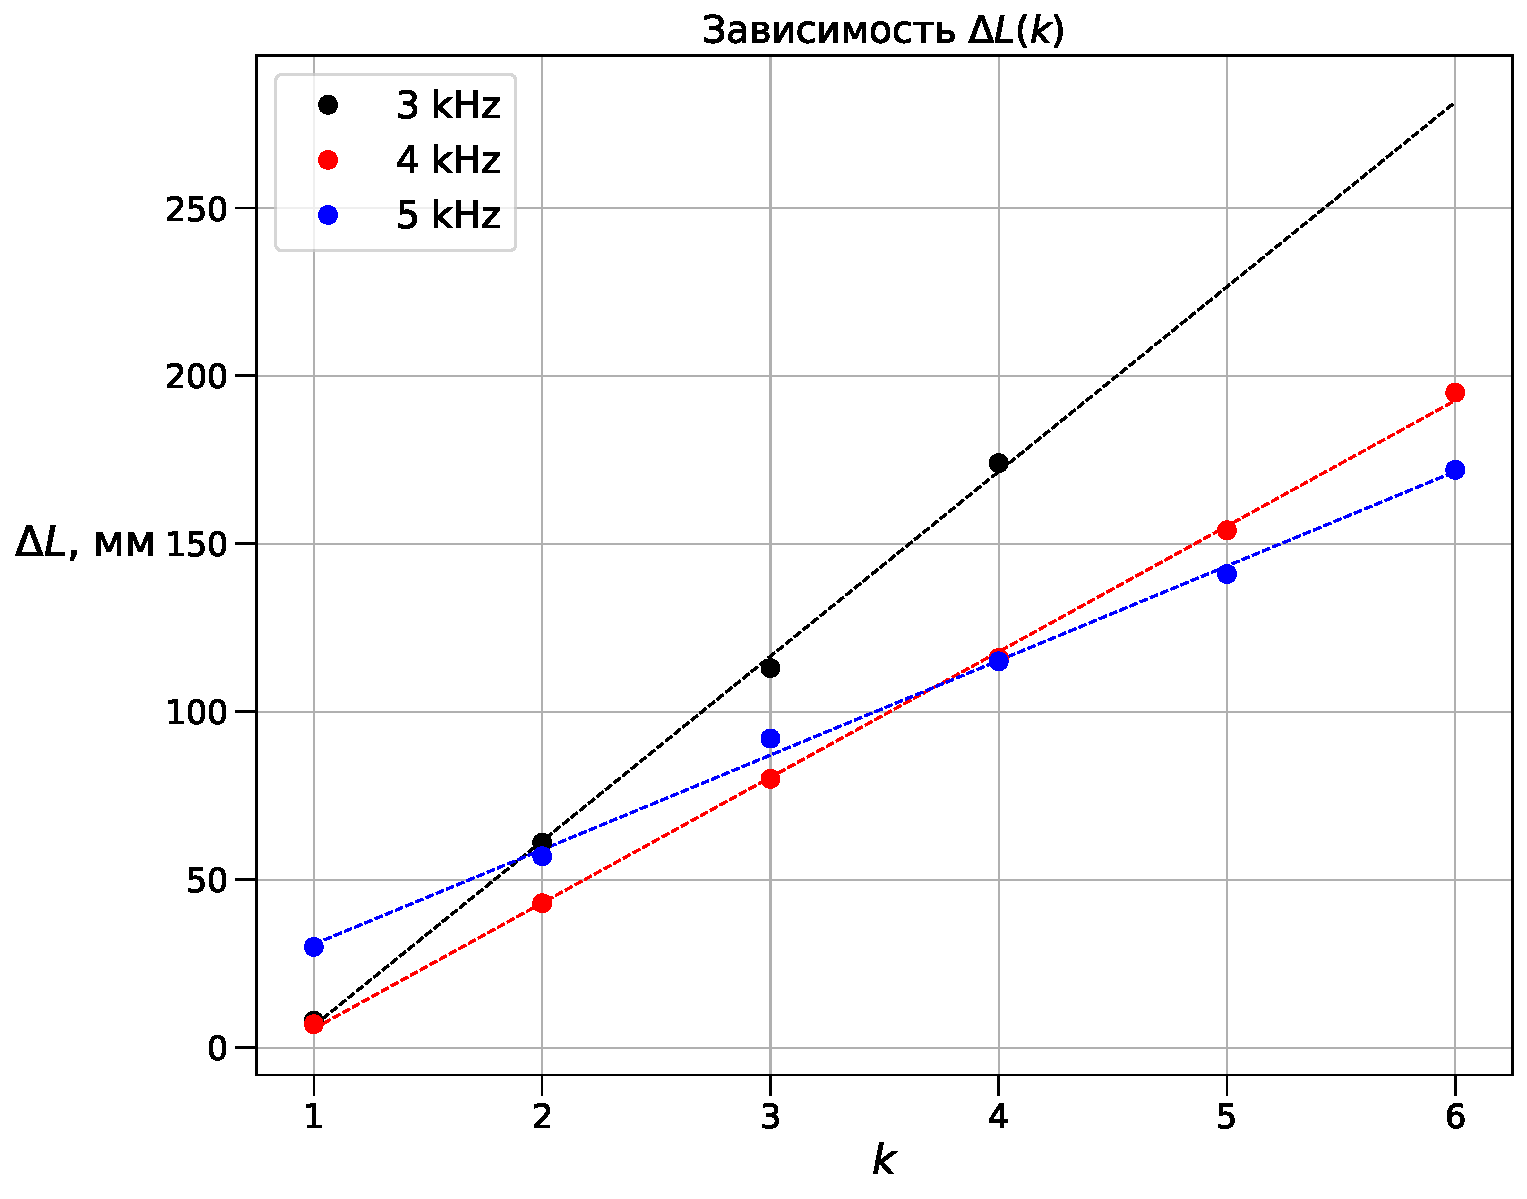
\includegraphics[scale=0.65]{2.1.3/CO.pdf}
		\caption{\centering График зависимости удлинения трубы \\ от номера полученного резонанса для $CO_2$}
		\label{fig:CO}
	\end{center}
\end{figure}

Для каждого значения частоты найдём соответсвующий ей коэфициент наклона умножим его на удвоенную частоту. По этим данным построим график \ref{const} зависимости скорости от частоты.

\begin{figure}[H]
	\begin{center}
		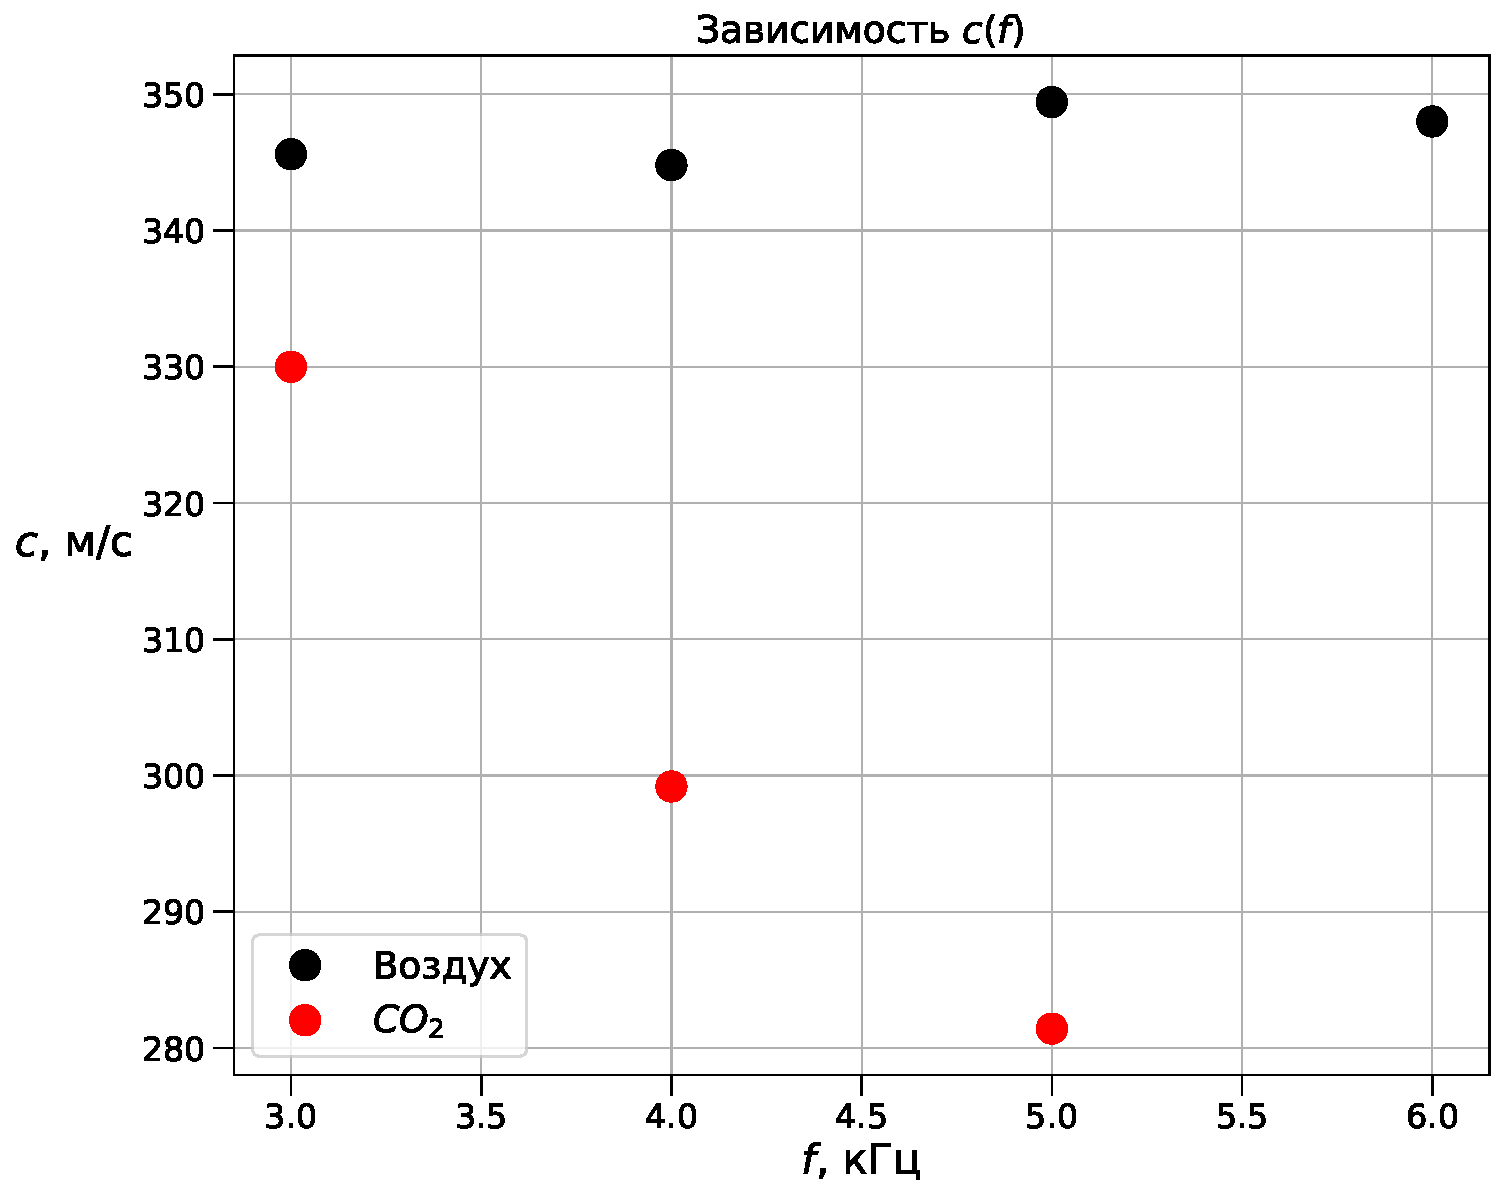
\includegraphics[scale=0.65]{2.1.3/c(f).pdf}
		\caption{График зависимости скорости звука от частоты}
		\label{const}
	\end{center}
\end{figure}

По графику видно, что для воздуха эта скорость является константой и равна $c_{\text{возд}}= 347 \pm 3$ м$/$с. Для углекислого газа наблюдается слишком большой разброс точек для определения скорости звука газе. Это свидетельствует о неудачной методике эксперимента или ошибке экспериментатора во время получения данных.

По формуле \ref{gamma} найдём соотношение $\displaystyle C_p/C_v$:

\begin{center}
    
    $\displaystyle \gamma=1,41 \pm 0,02$
    
\end{center}
Это соответствует табличным данным в пределах погрешности.

По данным таблицы 2 построим график (\ref{nu(k)}) зависимости $f_{k+1} - f_1$ от номера резонанса при различных температурах. 

\begin{figure}[H]
	\begin{center}
		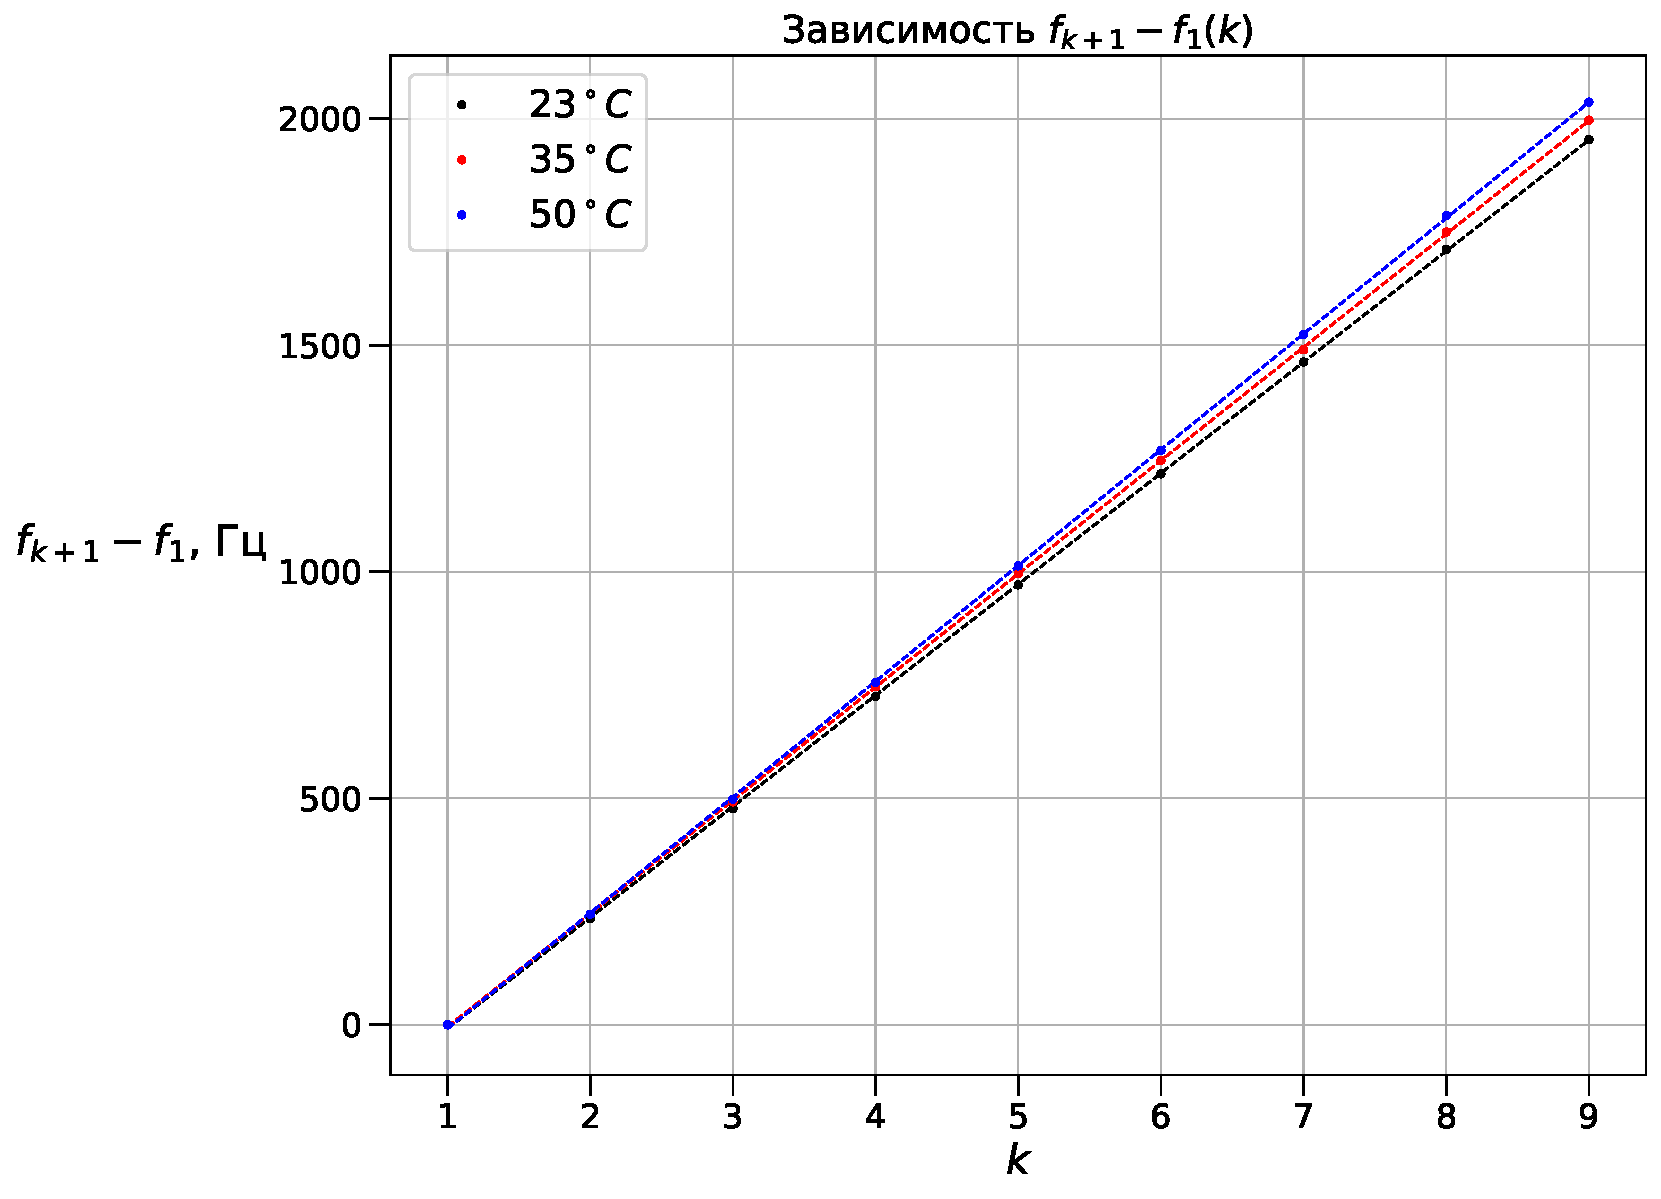
\includegraphics[scale=0.6]{2.1.3/nu(k).pdf}
		\caption{График зависимости $f_{k+1} - f_1$ от номера резонанса при различных температурах}
		\label{nu(k)}
	\end{center}
\end{figure}

По наклону графика найдём скорость звука для каждой температуры:

\begin{center}
    $\displaystyle c_{23}=343,3 \pm 0,7$ м$/$с 
    \break
    
    $\displaystyle c_{35}=350,0 \pm 0,6$ м$/$с 
    \break
    
    $\displaystyle c_{50}=357,8 \pm 0,7$ м$/$с 
    \break
\end{center}

По формуле \ref{gamma} найдём $\displaystyle C_p/C_v$:

\begin{center}
    
    $\displaystyle \gamma_{23}=1,39 \pm 0,01$
    \break
    
    $\displaystyle \gamma_{35}=1,39 \pm 0,01$
    \break
    
    $\displaystyle \gamma_{50}=1,38 \pm 0,01$
    \break
\end{center}


\end{document}
